%%%%%%%%%%%%%%%%%%%%%%%%%%%%%%
%
% Physics Lab Report #1
% Ver 1
% 09.01.2017
% Author: Abdollah Shajadi
% Teacher: Susanna Kujanpää
% 
%  OAMK | DIN16SP 
%
%%%%%%%%%%%%%%%%%%%%%%%%%%%%%%

%------------------------------
% Packages and configurations
%------------------------------

\documentclass[a4paper, 12pt]{article}
\usepackage[T1]{fontenc}
\usepackage[utf8]{inputenc}
\usepackage[a4paper, top=1in, bottom=1.5in, left=1in, right=1in]{geometry}
\usepackage{fancyhdr}
\pagestyle{fancy}
\fancyhf{}
\renewcommand{\headrulewidth}{0pt}
\renewcommand{\footrulewidth}{0pt}
\fancyhead[L]{}
\fancyhead[R]{
	
\includegraphics[width=3cm]{oamk.jpg}
}
\rfoot{\thepage}
\usepackage[protrusion=true,expansion=true]{microtype}
\usepackage{graphicx}
\usepackage{caption}
\usepackage{subcaption}
\usepackage{amsmath}
\usepackage{mathpazo}
\linespread{1.05}
\makeatletter
\renewcommand\@biblabel[1]{\textbf{#1.}}
\renewcommand{\@listI}{\itemsep=0pt}

\renewcommand{\maketitle}{ 
	\begin{flushright} 

		{\LARGE\@title} 
		
		\vspace{80pt} 
		
		{\large\@author} 
		
		\vspace{170pt} 
	\end{flushright}
}

%------------------------------
%  Title 
%------------------------------
\vspace*{\fill}
\title{\textbf{Physics Lab Report Work 1}\\
	Determination of the density of the body} 

\author{\textsc{Author: Abdollah Shajadi}
	\\{\textsc{Teacher: Susanna Kujanp{\"a}{\"a}}}
	\\{\textsc{Team members: Abdollah Shajadi, Yulia Yuvminina}}
	\\{\textsc{Date of work: 27.01.2017}}
	\\{\textsc{Date of return: 10.02.2017}}
	\\{\textsc{DIN16SP}}}

\begin{document}
	
	\maketitle 
	
\clearpage

\tableofcontents

\clearpage
%------------------------------
%  Summary and Keywords 
%------------------------------

\renewcommand{\abstractname}{Summary} 

\begin{abstract}

In this Lab work we measure and determine the density of rectangular parallelogram and cylinder.
we will measure the weight of parallelogram and cylinder with balance scale in air and then only parallelogram also in water and unknown liquid (alcohol), with 10 time measurements of diameter of the base and the height for cylinder and 3 sides of parallelogram we calculate the density. 
In the following pages comes the theory, calculations, formulas and the measures.

\end{abstract}

\hspace*{3,6mm}\textit{Keywords:} Density, Measurements, Micrometer, Caliper, Error estimation 

\vspace{30pt}

%------------------------------
%	Body
%------------------------------

\section{Theory}

Density (\(\rho\)) is defined by following equation where \(m\) is mass and \(v\) is volume of the body.

\[\rho = \dfrac{m}{v}\]

According to Archimedes' principle if the weight of the water displaced is less than the weight of the object, the object will sink, Otherwise the object will float, with the weight of the water displaced equal to the weight of the object. \cite{weber}
As described the buoyancy is equal to weight of displaced fluid in Archimedes' principle.

\[
\rho = \frac{m_{a}}{m_{a}-m_{l}}.\rho_{l}
\]

Where \(m_{a}\) is mass of the body that measured surrounded by air and \(m_{l}\) is mass of the body measured surrounded by liquid and \(\rho_{l}\) is density fo the liquid.

For Calculating density of rectangular parallelogram according to density formula and \(v=abc\) we get:

\[\rho = \frac{m_{1}}{abc} \]

And for the Cylinder we substitute \(v\) in density formula \(v = \frac{\pi d^{2} h}{4} \) .

%------------------------------

\section{Equipments}

We used a variety of different equipments, the following list is the main tools we used for the tasks.

\begin{figure}
	\centering
	\begin{minipage}{.5\textwidth}
		\centering
		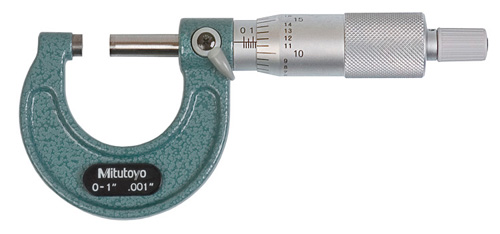
\includegraphics[width=.4\linewidth]{micrometer.jpg}
		\captionof{figure}{Micrometer}
	\end{minipage}%
	\begin{minipage}{.5\textwidth}
		\centering
		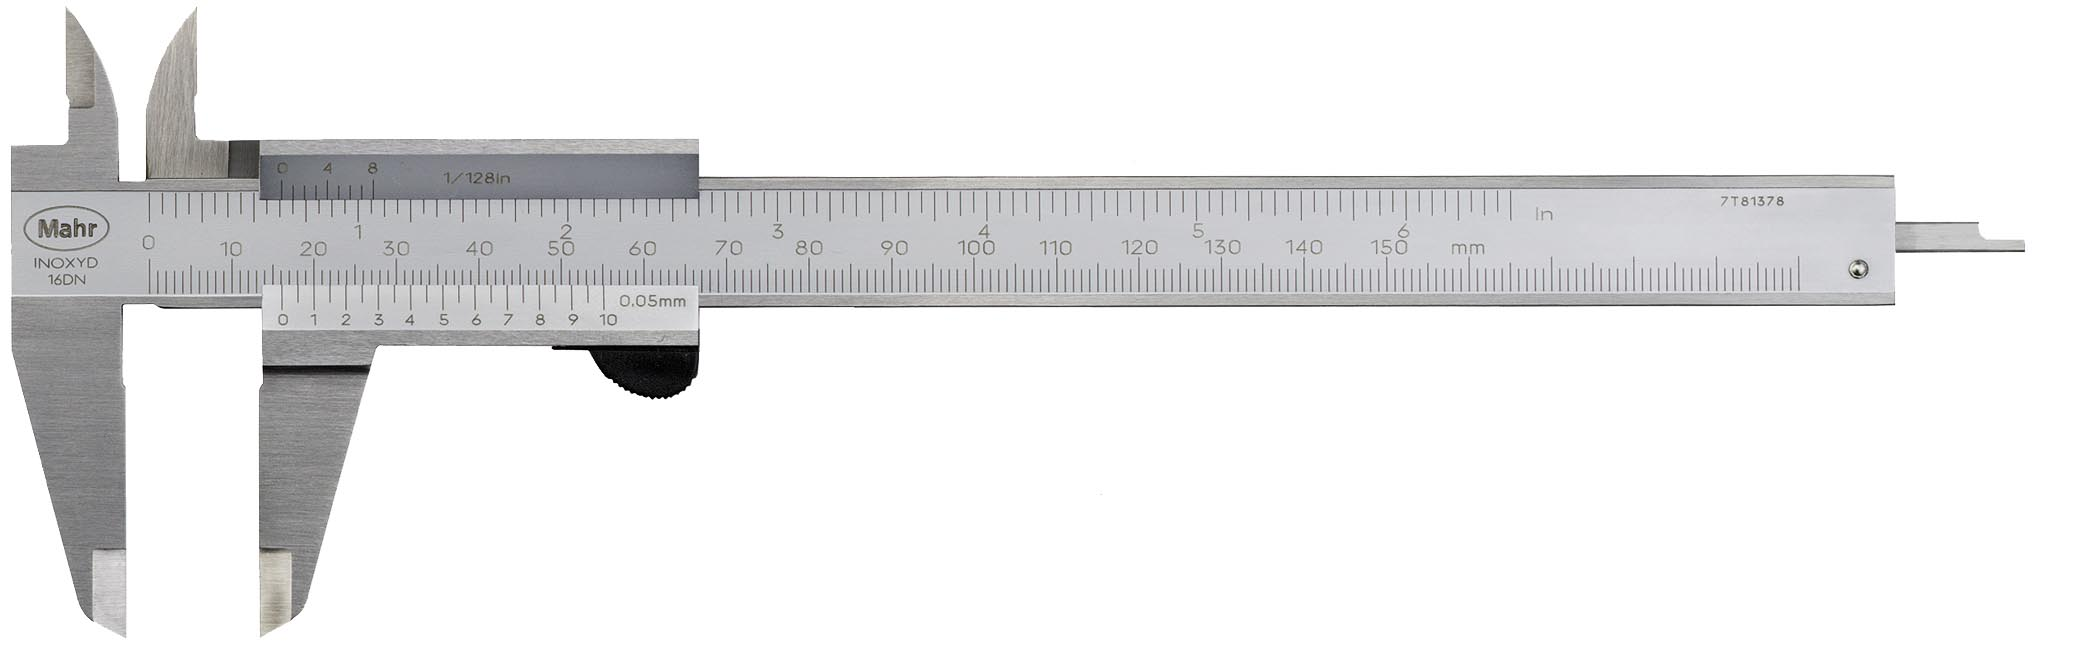
\includegraphics[width=.4\linewidth]{caliper.jpg}
		\captionof{figure}{Caliper}
	\end{minipage}
\end{figure}

\begin{enumerate}
	\item Micrometer (Figure 1)
	\item Caliper (Figure 2)
	\item Balance Scale
	\item Aerometer
	\item Water
	\item Alcohol (as unknown liquid)
	\item String
	\item Metal parallelogram
	\item Metal Cylinder
	\item Beaker
\end{enumerate}

%------------------------------
\section{Measurments and Calculations}

All the measurements and calculations are based on the work 1 formulas and instruction paper and signed result paper can be found on the last page of this report. on the following sections comes the detailed calculations of the lab.

\subsection{Density of rectangular parallelogram}

For the rectangular parallelogram we measured 3 sides of a, b and c for 10 times with Micrometer, following table shows the results of the measurements.

\begin{center}
	\begin{tabular}{||c c c c||} 
		\hline
		   &  a\((mm)\) & b\((mm)\)  &  c\((mm)\)  \\ [0.5ex] 
		\hline\hline
		1 & 20.00 & 20.01 & 14.40 \\ 
		\hline
		2 & 20.01 & 20.00 & 14.38 \\
		\hline
		3 & 20.00 & 20.00 & 14.45 \\
		\hline
		4 & 19.98 & 20.02 & 14.47 \\
		\hline
		5 & 20.00 & 20.01 & 14.44 \\
		\hline
		6 & 20.00 & 20.00 & 14.39 \\
		\hline
		7 & 20.02 & 19.99 & 14.39 \\
		\hline
		8 & 19.99 & 20.00 & 14.42 \\
		\hline
		9 & 20.00 & 19.98 & 14.49 \\
		\hline
		10 & 20.00 & 19.99 &  14.37 \\ [1ex] 
		\hline
	\end{tabular}
\end{center}

And using balance scale we got \(m_{1}\)= 43.90\(mm\) with the accuracy of \(\varDelta m\)= 0.01\(g\). and according to density formula we have:

\[
\rho = \dfrac{m}{v} = \dfrac{m}{abc} = \dfrac{43.90g}{20_{mm}.20_{mm}.14.42_{mm}} = \dfrac{43.90g}{5768_{mm^{3}}} \approx 0.0076_{\frac{g}{m^{3}}}
\]

\subsection{Density of cylinder}

We measured height and diameter with Caliper the following table shows the result of the measurements.

\begin{center}
	\begin{tabular}{||c c c||} 
		\hline
		&  h\((mm)\) & d\((mm)\)  \\ [0.5ex] 
		\hline\hline
		1 & 24.90 & 18.00 \\ 
		\hline
		2 & 24.70 & 17.95 \\
		\hline
		3 & 24.40 & 17.90 \\
		\hline
		4 & 24.30 & 18.10 \\
		\hline
		5 & 24.40 & 18.00 \\
		\hline
		6 & 24.60 & 17.95 \\
		\hline
		7 & 24.70 & 18.20 \\
		\hline
		8 & 24.70 & 18.10 \\
		\hline
		9 & 24.40 & 17.90  \\
		\hline
		10 & 24.50 & 18.00 \\ [1ex] 
		\hline
	\end{tabular}
\end{center}

\subsection{Density of unknown liquid}



%------------------------------
\section{Error estimation}



%------------------------------
\section{Conclusion}



%------------------------------
% Bibliography
%------------------------------

\addcontentsline{toc}{section}{References}
\bibliographystyle{unsrt}
\bibliography{physlab1}

%------------------------------

\end{document}


